In questo capitolo richiamiamo gli strumenti teorici usati nel resto della tesi. Non pretendiamo di essere esaustivi: per una trattazione completa si rimanda a \cite{goodfellow2016deep}. L'obiettivo è fissare la notazione e mettere in evidenza i punti che diventeranno importanti quando sostituiremo le matrici dense con matrici strutturate. Il più importante tra questi è il fatto che, in un Transformer, quasi tutti i parametri e quasi tutto il tempo di esecuzione si concentrano nei prodotti tra una matrice di pesi e un vettore di attivazioni.

\section{Modelli linguistici autoregressivi}

Sia $\mathcal{V}$ un vocabolario finito di simboli, che chiameremo \emph{token}, e sia $x=(x_1,\dots,x_T)$ una sequenza di token. Un modello linguistico autoregressivo scompone la probabilità della sequenza nel prodotto delle probabilità condizionate di ciascun token dato il prefisso che lo precede:
\begin{equation}
p_\theta(x) = \prod_{t=1}^{T} p_\theta(x_t \mid x_{<t}),
\end{equation}
dove $\theta$ indica l'insieme dei parametri. La scomposizione è esatta per qualunque distribuzione; ciò che la rende utile è la scelta di una funzione parametrica, la rete neurale, che calcola ogni fattore a partire dal prefisso.

\subsection{Log-verosimiglianza negativa e perplessità}

Il modello si addestra massimizzando la probabilità dei testi di addestramento, o, in modo equivalente, minimizzando la log-verosimiglianza negativa media per token:
\begin{equation}
\mathcal{L}(\theta) = -\frac{1}{|\mathcal{I}|}\sum_{t\in\mathcal{I}} \log p_\theta(x_{t}\mid x_{<t}),
\label{eq:nll}
\end{equation}
dove $\mathcal{I}$ è l'insieme delle posizioni su cui si calcola la perdita. Nel seguito indicheremo questa quantità con l'acronimo NLL (\emph{negative log-likelihood}) e la misureremo in \emph{nat}, cioè con il logaritmo naturale. La NLL coincide con l'entropia incrociata tra la distribuzione empirica del testo e quella del modello.

Due grandezze derivate sono di uso comune. La \emph{perplessità} è l'esponenziale della NLL, $\mathrm{PPL}=e^{\mathcal{L}}$, e si può leggere come il numero di scelte equiprobabili tra cui il modello è in media incerto a ogni passo. I \emph{bit per byte} (BPC o BPB) dividono la perdita totale, espressa in bit, per il numero di byte del testo; hanno il pregio di non dipendere dal tokenizzatore e permettono di confrontare modelli con vocabolari diversi.

È bene ricordare fin d'ora che una NLL bassa non garantisce testi di qualità. La NLL misura quanto il modello sia sorpreso dal testo reale quando legge il prefisso corretto (\emph{teacher forcing}); la generazione, invece, procede con i token che il modello stesso ha scelto, e un piccolo errore può propagarsi. Per questo nella tesi misureremo separatamente la capacità predittiva e la qualità dei testi generati.

\subsection{Tokenizzazione}

I modelli moderni non lavorano né su caratteri né su parole intere, ma su frammenti di parola ottenuti con l'algoritmo \emph{Byte Pair Encoding} (BPE) \cite{sennrich2016neural}. Si parte dall'alfabeto dei byte e si fondono ripetutamente le coppie di simboli adiacenti più frequenti nel corpus, fino a raggiungere la dimensione di vocabolario desiderata. Le parole comuni finiscono per avere un token proprio, quelle rare vengono spezzate in più parti, e nessuna stringa resta impossibile da rappresentare.

La dimensione del vocabolario ha un effetto diretto sul numero di parametri. La matrice di \emph{embedding}, che associa a ogni token un vettore, ha $|\mathcal{V}|\times d$ elementi, dove $d$ è la dimensione nascosta del modello. In un modello piccolo questa matrice può rappresentare una frazione rilevante del totale. I modelli confrontati in questa tesi usano tutti lo stesso tokenizzatore BPE, con \num{50257} token: la matrice di embedding di STERA 30M è quindi la più grande del modello, ed è anch'essa rappresentata con blocchi strutturati.

\section{L'architettura Transformer}

Il Transformer è stato introdotto da Vaswani e collaboratori in \emph{Attention Is All You Need} \cite{vaswani2017attention} come architettura composta da un \emph{encoder} e da un \emph{decoder}. La Figura~\ref{fig:transformer-originale-vaswani} ne riproduce il diagramma originale, con l'encoder sulla sinistra e il decoder sulla destra.

\begin{figure}[htbp]
\centering
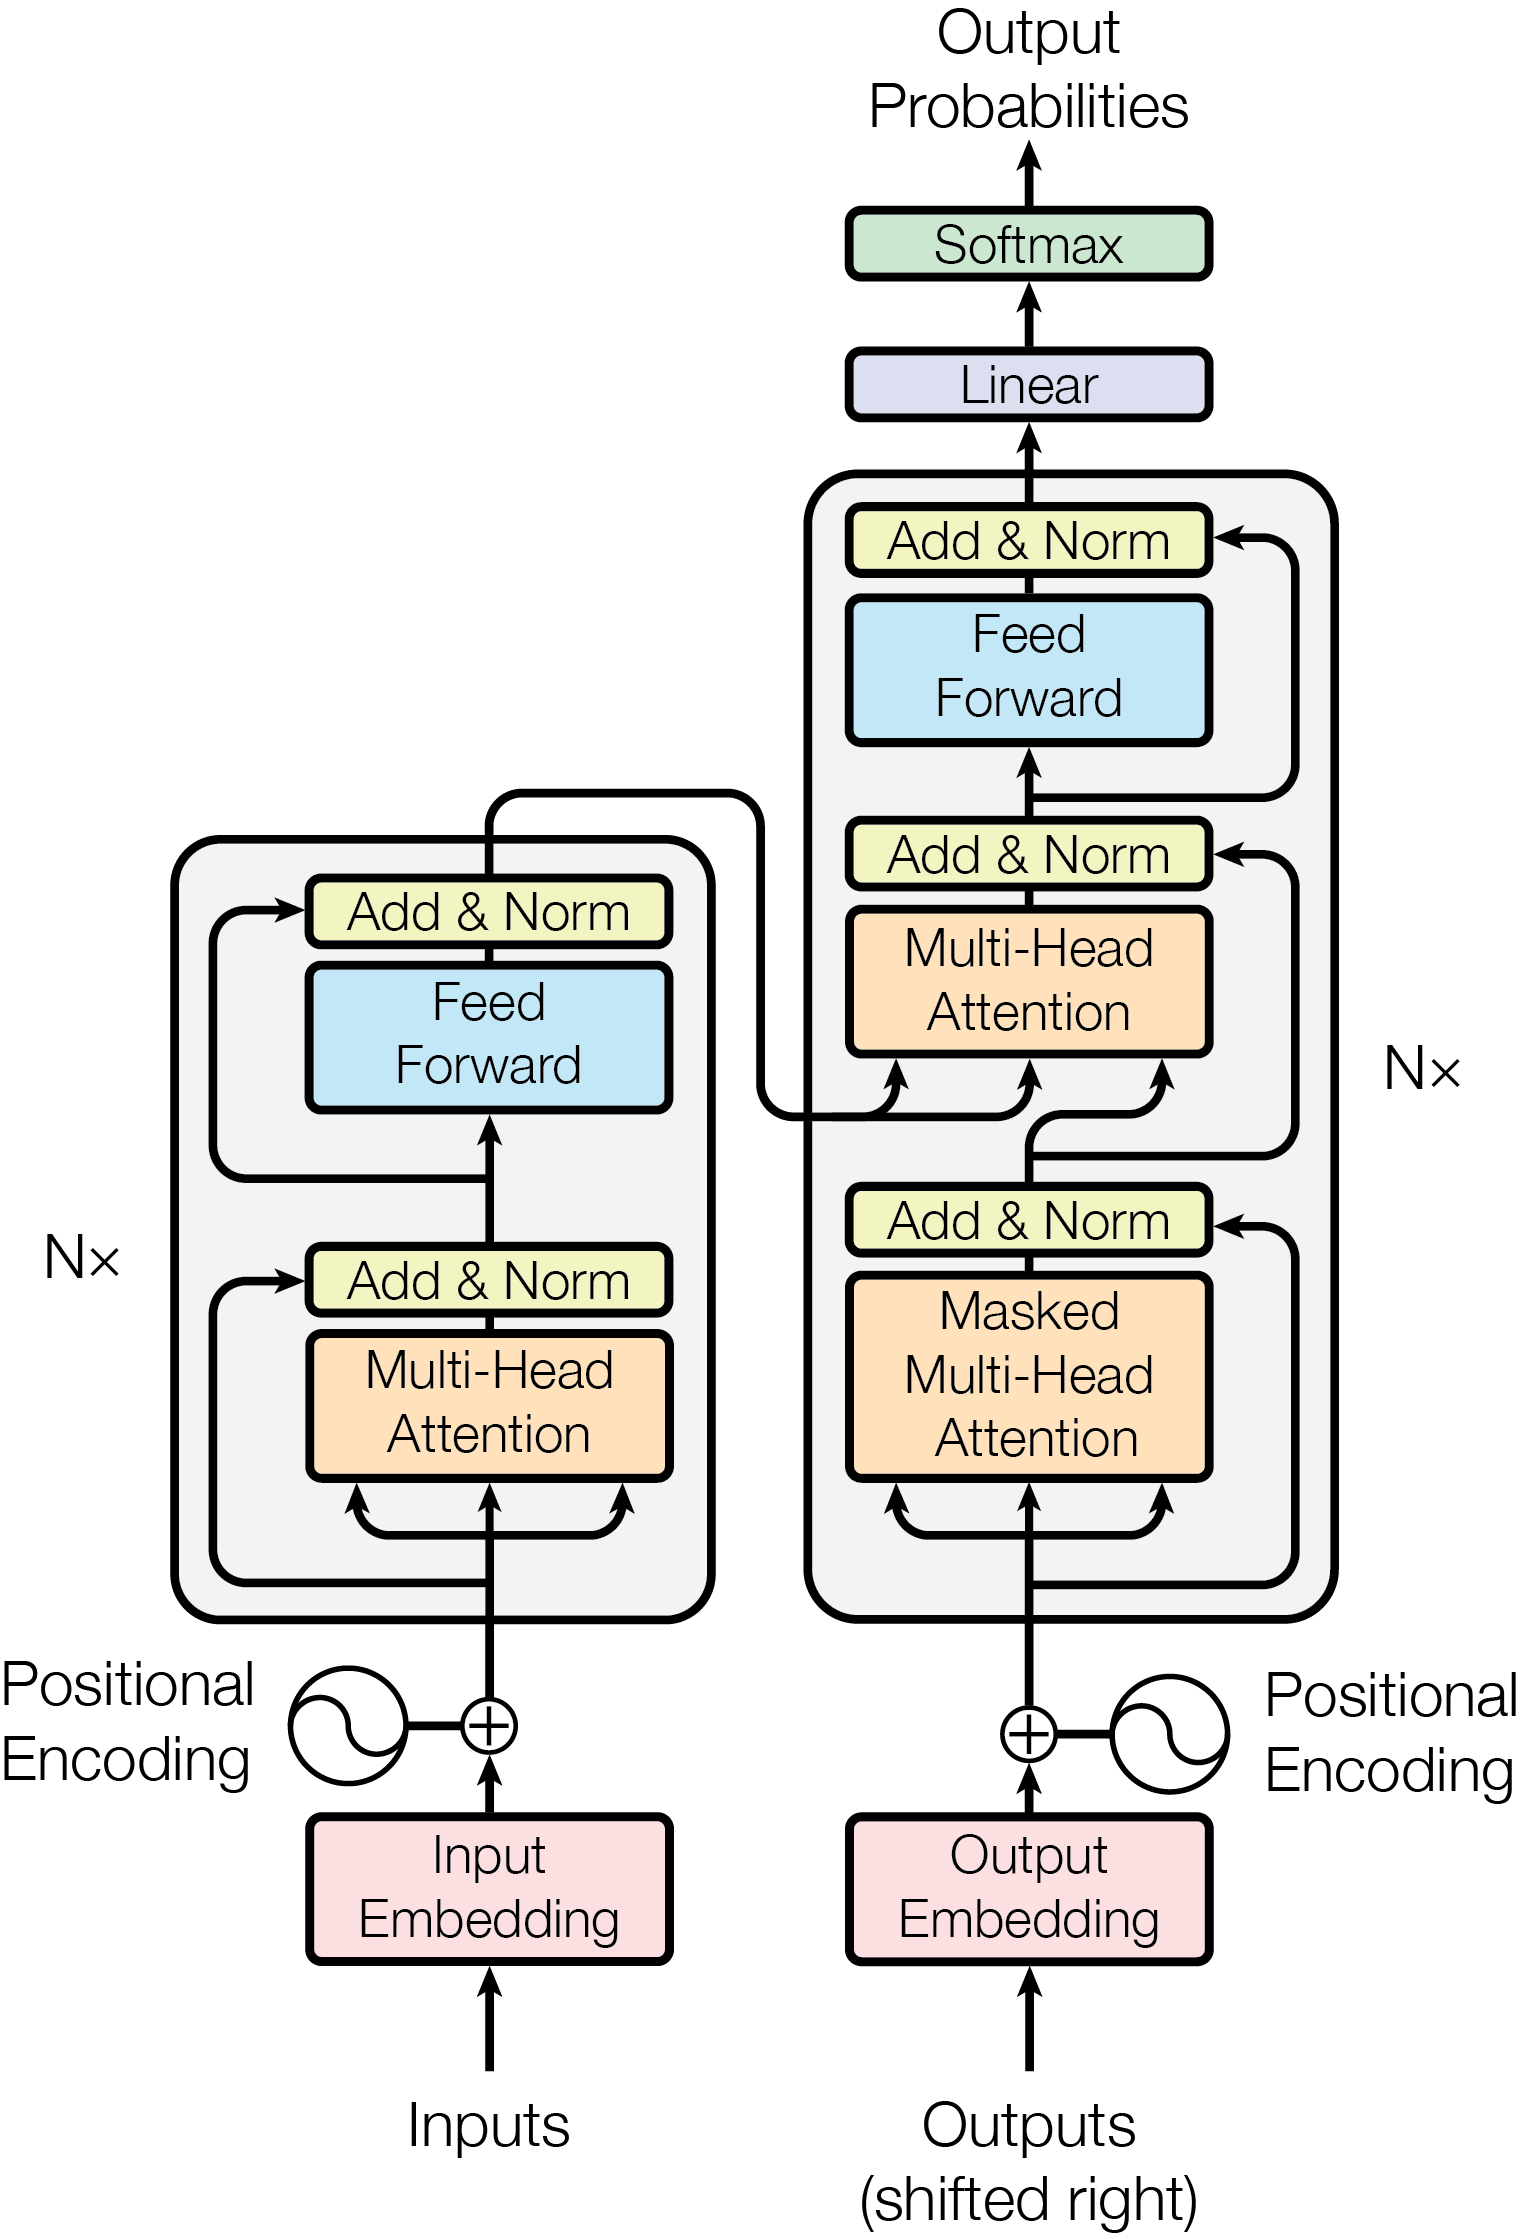
\includegraphics[width=.66\linewidth,height=.69\textheight,keepaspectratio]{figure/origini/transformer_vaswani2017_fig1_originale.png}
\caption{Architettura originale del Transformer encoder--decoder. Riproduzione della Figura~1 di Vaswani et al., \emph{Attention Is All You Need} (2017) \cite{vaswani2017attention}; fonte originale: arXiv:1706.03762. Figura riprodotta per finalità accademiche con attribuzione, secondo l'autorizzazione indicata nel paper.}
\label{fig:transformer-originale-vaswani}
\end{figure}

L'encoder originale è una pila di moduli di \emph{self-attention} e reti feed-forward, intervallati da normalizzazioni e connessioni residue. Il decoder utilizza un'attenzione causale (nel diagramma, \emph{Masked Multi-Head Attention}) e un ulteriore blocco di \emph{cross-attention} sui risultati dell'encoder. I simboli $N\times$ indicano la ripetizione dei blocchi. Lo schema riguarda il Transformer storico, non una rappresentazione delle dimensioni o dei pesi di STERA.

I modelli linguistici autoregressivi della famiglia GPT utilizzano prevalentemente una variante \emph{decoder-only} \cite{radford2019language}: conservano i blocchi di attenzione causale e il feed-forward, ma non hanno un encoder separato e non necessitano dello strato di cross-attention encoder--decoder mostrato in Figura~\ref{fig:transformer-originale-vaswani}. Questa è anche l'impostazione generale di \textbf{STERA 30M}, che impiega normalizzazione pre-residuale e posizioni apprese. La sua architettura specifica, con sei strati, sedici teste e proiezioni RowMask23, è documentata nel diagramma dedicato della Figura~\ref{fig:stera30m-flusso}; non va confusa con il diagramma del paper del 2017. Descriviamo i suoi componenti nell'ordine in cui vengono attraversati.

\subsection{Embedding e posizione}

Ogni token $x_t$ viene sostituito dalla riga corrispondente della matrice di embedding $E\in\mathbb{R}^{|\mathcal{V}|\times d}$. Poiché l'attenzione, da sola, non distingue l'ordine degli elementi, serve un'informazione di posizione. Le varianti più semplici sommano all'embedding un secondo vettore appreso che dipende dalla posizione $t$. Una soluzione più recente, le \emph{Rotary Position Embeddings} (RoPE) \cite{su2024roformer}, ruota le componenti delle query e delle chiavi di un angolo proporzionale alla posizione, in modo che il prodotto scalare tra due posizioni dipenda solo dalla loro distanza relativa. STERA 30M adotta la soluzione più semplice, con vettori di posizione appresi, come i modelli TinyStories con cui è confrontato.

\subsection{Attenzione causale a più teste}

Sia $H\in\mathbb{R}^{T\times d}$ la matrice degli stati in ingresso a un blocco. L'attenzione calcola tre proiezioni lineari,
\begin{equation}
Q = H W_Q^\top,\qquad K = H W_K^\top,\qquad V = H W_V^\top,
\end{equation}
con $W_Q,W_K,W_V\in\mathbb{R}^{d\times d}$. Le righe di $Q$ e $K$ vengono confrontate tramite prodotto scalare, e il risultato, normalizzato, decide quanto ogni posizione debba ``guardare'' le altre:
\begin{equation}
\mathrm{Attn}(Q,K,V) = \mathrm{softmax}\!\left(\frac{QK^\top}{\sqrt{d_h}} + M\right) V .
\end{equation}
La matrice $M$ è la \emph{maschera causale}: vale $0$ se $j\le t$ e $-\infty$ altrimenti, così che la posizione $t$ non possa vedere i token futuri. Senza questa maschera il modello imparerebbe a copiare la risposta invece di prevederla.

Nella versione a più teste il vettore di dimensione $d$ viene diviso in $h$ blocchi di dimensione $d_h=d/h$, ognuno dei quali esegue un'attenzione indipendente. I risultati vengono concatenati e passati per una quarta proiezione $W_O\in\mathbb{R}^{d\times d}$. Le teste permettono al modello di seguire contemporaneamente relazioni diverse, per esempio il soggetto di una frase e il personaggio introdotto qualche riga prima.

\subsection{Blocco feed-forward}

Dopo l'attenzione, ogni posizione attraversa indipendentemente una piccola rete a due strati:
\begin{equation}
\mathrm{FFN}(h) = W_2\,\phi(W_1 h + b_1) + b_2,
\end{equation}
con $W_1\in\mathbb{R}^{f\times d}$, $W_2\in\mathbb{R}^{d\times f}$ e tipicamente $f=4d$. La funzione di attivazione $\phi$ è di solito la GELU \cite{hendrycks2016gelu}, una versione smussata della ReLU. Il blocco feed-forward contiene circa due terzi dei parametri di ogni strato.

\subsection{Normalizzazione e connessioni residue}

Ogni sotto-blocco è preceduto da una normalizzazione e racchiuso in una connessione residua:
\begin{align}
h' &= h + \mathrm{Attn}(\mathrm{LN}(h)),\\
h'' &= h' + \mathrm{FFN}(\mathrm{LN}(h')).
\end{align}
La \emph{Layer Normalization} \cite{ba2016layer} riporta ogni vettore a media nulla e varianza unitaria e poi applica un guadagno e uno spostamento appresi. Le connessioni residue fanno sì che il gradiente possa attraversare molti strati senza svanire, e rendono stabile l'addestramento di reti profonde.

\subsection{Testa di uscita}

Dopo l'ultimo blocco, una normalizzazione finale e una proiezione lineare producono un vettore di \emph{logit}, uno per ogni token del vocabolario. Spesso la matrice di questa proiezione coincide con la matrice di embedding trasposta (\emph{weight tying}) \cite{press2017using}: si risparmiano parametri e si ottiene di solito un modello migliore. La funzione softmax trasforma infine i logit in una distribuzione di probabilità sul token successivo.

\subsection{Dove stanno i parametri}

Conviene fare il conto dei parametri di uno strato. Le quattro proiezioni dell'attenzione contribuiscono con $4d^2$ valori, il blocco feed-forward con $2df=8d^2$. Le normalizzazioni e i bias aggiungono un numero di valori proporzionale a $d$, trascurabile. In totale ogni strato contiene circa $12d^2$ parametri, e \emph{tutti} quelli significativi stanno in sei matrici dense. Lo stesso vale per il tempo di calcolo durante la generazione: a ogni token ciascuna di quelle matrici viene moltiplicata per un vettore.

Questa osservazione è il punto di partenza della tesi. Se si vuole cambiare in modo sostanziale l'ingombro e la velocità di un Transformer, bisogna intervenire sulle sue matrici lineari. Il resto dell'architettura (attenzione, normalizzazioni, funzioni di attivazione) può restare invariato.

\section{Addestramento}

\subsection{Retropropagazione in uno strato lineare}

L'addestramento usa la discesa del gradiente: si calcola la derivata della perdita rispetto a ogni parametro e si sposta il parametro nella direzione opposta. Il gradiente si ottiene con la retropropagazione, cioè applicando la regola della catena all'indietro attraverso la rete.

Per uno strato lineare $Y=XW^\top$, con $X\in\mathbb{R}^{B\times n}$ ingressi, $W\in\mathbb{R}^{m\times n}$ pesi e $Y\in\mathbb{R}^{B\times m}$ uscite, se $G_Y=\partial\mathcal{L}/\partial Y$ è il gradiente che arriva dall'alto, valgono
\begin{equation}
\frac{\partial\mathcal{L}}{\partial W} = G_Y^\top X,\qquad
\frac{\partial\mathcal{L}}{\partial X} = G_Y W.
\label{eq:linear-grad}
\end{equation}
La prima formula fornisce il gradiente dei pesi, la seconda il gradiente da passare allo strato precedente. Nel Capitolo~\ref{cap:capitoli/03-formalismo} useremo la prima per ricavare il gradiente rispetto alle coordinate compresse: basterà comporla con la derivata della mappa che costruisce $W$ dalle coordinate.

\subsection{Adam e AdamW}

La discesa del gradiente semplice usa un unico passo per tutti i parametri. Adam \cite{kingma2015adam} adatta invece il passo a ciascun parametro, mantenendo una media esponenziale del gradiente e del suo quadrato:
\begin{align}
m_t &= \beta_1 m_{t-1} + (1-\beta_1) g_t,\\
v_t &= \beta_2 v_{t-1} + (1-\beta_2) g_t^2,\\
\theta_{t+1} &= \theta_t - \eta_t\,\frac{\hat m_t}{\sqrt{\hat v_t}+\epsilon},
\end{align}
dove $\hat m_t=m_t/(1-\beta_1^t)$ e $\hat v_t=v_t/(1-\beta_2^t)$ correggono la distorsione iniziale dovuta all'inizializzazione a zero. AdamW \cite{loshchilov2019decoupled} aggiunge un termine di decadimento dei pesi separato dal gradiente, $-\eta_t\lambda\theta_t$, che agisce come regolarizzazione. Per STERA 30M usiamo $\beta_1=0{,}9$, $\beta_2=0{,}95$ e $\lambda=0{,}1$ (Sezione~\ref{sec:stera30m-config-training}).

Ogni parametro allenabile richiede quindi due valori aggiuntivi nello stato dell'ottimizzatore. È per questo che ridurre il numero di parametri allenabili riduce in proporzione anche la memoria dell'addestramento.

\subsection{Tasso di apprendimento e stabilità}

Il tasso di apprendimento $\eta_t$ non è costante. Nei primi passi cresce linearmente da zero (\emph{warmup}), così che i momenti di Adam abbiano il tempo di stimarsi; poi resta costante o decresce, per esempio seguendo un coseno o una rampa lineare, fino a una frazione del valore massimo. Il profilo usato per STERA 30M è descritto nella Sezione~\ref{sec:stera30m-config-training}. Per evitare che un singolo lotto anomalo produca un passo troppo grande, la norma complessiva del gradiente viene limitata a un valore massimo (\emph{gradient clipping}) \cite{pascanu2013difficulty}.

\section{Generazione del testo}

Un modello addestrato fornisce, dato un prefisso, una distribuzione sul token successivo. Per generare un testo si sceglie un token, lo si aggiunge al prefisso e si ripete. Il modo in cui si sceglie il token è detto \emph{strategia di decodifica} e ha un effetto rilevante sulla qualità.

La scelta più semplice è prendere sempre il token più probabile (\emph{greedy}). Il testo che ne risulta è spesso ripetitivo, perché il modello tende a ricadere nelle stesse frasi. Il campionamento introduce varietà. La \emph{temperatura} $\tau$ divide i logit prima della softmax: valori minori di uno concentrano la probabilità sui token migliori, valori maggiori la distribuiscono. Il campionamento \emph{top-$k$} \cite{fan2018hierarchical} limita la scelta ai $k$ token più probabili; il campionamento \emph{nucleus} o \emph{top-$p$} \cite{holtzman2020curious} sceglie il più piccolo insieme di token la cui probabilità cumulata supera $p$. A queste regole si possono aggiungere penalità per le ripetizioni.

Nelle valutazioni di questa tesi tutti i modelli generano con campionamento top-$k$, $k=40$, e temperatura $0{,}75$.

\subsection{Cache di chiavi e valori}

Durante la generazione, il prefisso cresce di un token alla volta. Ricalcolare ogni volta l'attenzione sull'intero prefisso sarebbe uno spreco: le chiavi e i valori delle posizioni passate non cambiano. Si conservano quindi in una \emph{KV cache} e, a ogni nuovo token, si calcolano solo la query, la chiave e il valore della nuova posizione. Il costo per token diventa dominato, ancora una volta, dai prodotti matrice--vettore delle proiezioni lineari.

\section{Memoria e trasferimento dei pesi}
\label{sec:memoria-trasferimento}

\subsection{Una gerarchia di memorie}

Durante la generazione, ogni token richiede di applicare tutte le matrici del modello. I pesi devono quindi trovarsi in una memoria da cui l'unità di calcolo possa leggerli rapidamente. Un dispositivo dispone di più livelli di memoria, sempre più capienti e sempre più lenti (Figura~\ref{fig:gerarchia-memoria}): la memoria vicina all'unità di calcolo, la memoria principale e il disco. Sul Mac con chip M1 usato nella tesi, CPU e GPU condividono 16~GiB di memoria unificata, con una banda teorica di circa 68~GB/s; l'SSD interno offre circa 2,4~GB/s in lettura sequenziale (Sezione~\ref{sec:ssd-io-verificato}), quasi trenta volte meno.

\begin{figure}[htbp]
\centering
\begin{tikzpicture}[
  liv/.style={draw=steraGrigio, rounded corners=2pt, minimum height=9mm, align=center, font=\small},
  freccia/.style={-{Latex[length=2mm]}, thick, steraGrigio}]
\node[liv, minimum width=34mm, fill=steraBlu!12] (gpu) {Unità di calcolo\\{\footnotesize registri e cache}};
\node[liv, minimum width=62mm, fill=steraBlu!6, below=9mm of gpu] (ram) {Memoria principale (16 GiB)\\{\footnotesize pesi residenti, cache KV, attivazioni}};
\node[liv, minimum width=90mm, fill=white, below=11mm of ram] (ssd) {Disco SSD (centinaia di GB)\\{\footnotesize copia persistente di tutti i pesi}};
\draw[freccia] ([xshift=-6mm]ram.north) -- node[left, font=\footnotesize]{$\approx 68$ GB/s} ([xshift=-6mm]gpu.south);
\draw[freccia] ([xshift=-6mm]ssd.north) -- node[left, font=\footnotesize]{$\approx 2{,}4$ GB/s} ([xshift=-6mm]ram.south);
\draw[freccia, dashed] ([xshift=16mm]ram.south) -- node[left, font=\footnotesize]{swap-out} ([xshift=16mm]ssd.north);
\draw[freccia] ([xshift=24mm]ssd.north) -- node[right, font=\footnotesize]{swap-in} ([xshift=24mm]ram.south);
\end{tikzpicture}
\caption{Gerarchia di memoria di un dispositivo con memoria unificata. Le bande indicate sono quelle del Mac M1 usato nelle misure. Quando i pesi non entrano nella memoria principale, una parte resta sul disco e viene caricata (swap-in) prima dell'uso, mentre la memoria occupata da pesi non più necessari viene liberata (swap-out).}
\label{fig:gerarchia-memoria}
\end{figure}

\subsection{Pesi residenti e pesi trasferiti}

Se l'intero modello entra nella memoria principale, i pesi vengono caricati una volta e restano \emph{residenti}: ogni token paga solo il calcolo e la lettura dalla memoria principale. Se il modello è più grande della memoria disponibile, occorre una politica di \emph{swap}. Nella forma più semplice, il sistema operativo gestisce i pesi tramite memoria virtuale: il file dei pesi viene mappato in memoria e le pagine vengono lette dal disco quando servono e scartate quando la memoria si esaurisce. Le politiche specifiche per i modelli linguistici sfruttano invece la struttura della rete: poiché gli strati sono applicati in ordine, è possibile caricare uno strato (\emph{swap-in}) poco prima di usarlo e liberarne la memoria (\emph{swap-out}) subito dopo, mantenendo residenti solo le parti usate più spesso, come l'embedding e la testa di uscita.

\subsection{Costo di un token con pesi trasferiti}

Sia $B$ il numero di byte di pesi che devono essere letti dal disco per generare un token, $\beta$ la banda di lettura del disco e $T_c$ il tempo di calcolo del token. Se trasferimento e calcolo avvengono in sequenza, il tempo per token è
\begin{equation}
T_{\mathrm{seq}} = \frac{B}{\beta} + T_c .
\label{eq:tempo-sequenziale}
\end{equation}
Con il \emph{prefetch}, lo strato $\ell+1$ viene caricato mentre si calcola lo strato $\ell$, usando due aree di memoria alternate (\emph{doppio buffer}). Trasferimento e calcolo si sovrappongono e, a regime,
\begin{equation}
T_{\mathrm{pref}} \approx \max\!\left(\frac{B}{\beta},\,T_c\right).
\label{eq:tempo-prefetch}
\end{equation}
La Figura~\ref{fig:prefetch} confronta le due politiche. Nei modelli linguistici su dispositivi personali, in generazione con un solo testo alla volta, il calcolo per token è piccolo rispetto alla lettura dei pesi: il termine $B/\beta$ domina e il prefetch può nascondere al più il tempo di calcolo. L'unico modo di ridurre sostanzialmente il tempo per token è ridurre $B$, cioè leggere meno byte. È qui che si inserisce una rappresentazione compatta dei pesi: a parità di banda, ridurre di un fattore $r$ i byte da trasferire riduce dello stesso fattore il termine dominante, oppure permette di mantenere residente un modello che altrimenti andrebbe trasferito.

\begin{figure}[htbp]
\centering
\begin{tikzpicture}[x=9mm, y=6mm, font=\footnotesize]
\tikzset{car/.style={draw=steraBlu, fill=steraBlu!18}, cal/.style={draw=steraArancio, fill=steraArancio!22}}
\node[anchor=east] at (-0.2,3.5) {Sequenziale};
\node[anchor=east] at (-0.2,3.0) {\scriptsize disco};
\node[anchor=east] at (-0.2,2.2) {\scriptsize calcolo};
\foreach \i/\x in {1/0,2/3,3/6} {
  \draw[car] (\x,2.7) rectangle ++(2,0.6) node[midway]{$L_\i$};
  \draw[cal] (\x+2,1.9) rectangle ++(1,0.6) node[midway]{$L_\i$};
}
\node[anchor=east] at (-0.2,0.5) {Con prefetch};
\node[anchor=east] at (-0.2,0.0) {\scriptsize disco};
\node[anchor=east] at (-0.2,-0.8) {\scriptsize calcolo};
\foreach \i/\x in {1/0,2/2,3/4} {
  \draw[car] (\x,-0.3) rectangle ++(2,0.6) node[midway]{$L_\i$};
  \draw[cal] (\x+2,-1.1) rectangle ++(1,0.6) node[midway]{$L_\i$};
}
\draw[-{Latex[length=2mm]}, steraGrigio] (0,-1.7) -- (9.4,-1.7) node[right]{tempo};
\draw[decorate, decoration={brace, amplitude=3pt, mirror}, steraGrigio] (0,1.75) -- (9,1.75) node[midway, below=2pt]{$3\,(B_\ell/\beta + T_{c,\ell})$};
\draw[decorate, decoration={brace, amplitude=3pt, mirror}, steraGrigio] (0,-1.95) -- (7,-1.95) node[midway, below=2pt]{$3\,B_\ell/\beta + T_{c,\ell}$};
\end{tikzpicture}
\caption{Trasferimento degli strati dal disco per un token, con tre strati $L_1,L_2,L_3$. In alto ogni strato viene prima caricato e poi calcolato. In basso, con il prefetch, il caricamento dello strato successivo procede durante il calcolo di quello corrente: quando la lettura è più lenta del calcolo, il tempo è dominato dai byte da trasferire.}
\label{fig:prefetch}
\end{figure}

\section{Strumenti statistici}

Le differenze tra modelli che misureremo sono spesso piccole, e vanno accompagnate da una misura di incertezza. Richiamiamo i tre strumenti che useremo.

\paragraph{Bootstrap.} Per stimare l'intervallo di confidenza di una differenza media, per esempio tra la NLL di due modelli sugli stessi testi, si ricampionano con reinserimento le unità di valutazione, per esempio i racconti, e si ricalcola la differenza molte volte \cite{efron1979bootstrap}. I quantili $2{,}5\%$ e $97{,}5\%$ della distribuzione ottenuta danno un intervallo al 95\%.

\paragraph{Intervallo di Wilson.} Per una proporzione, come la frazione di storie giudicate corrette, l'intervallo di Wilson \cite{wilson1927probable} è più affidabile di quello basato sull'approssimazione normale quando la proporzione è vicina a zero o a uno o il campione è piccolo.

\paragraph{Test di McNemar.} Quando due modelli sono valutati sugli stessi incipit con un esito binario (storia corretta o no), le coppie in cui entrambi riescono o entrambi falliscono non dicono nulla sulla differenza fra i modelli. Il test esatto di McNemar \cite{mcnemar1947note} considera solo le coppie discordanti: indicato con $b$ il numero di incipit in cui riesce solo il primo modello e con $c$ quello in cui riesce solo il secondo, sotto l'ipotesi nulla di uguale prestazione $b$ segue una distribuzione binomiale con $n=b+c$ prove e probabilità $1/2$. Il valore $p$ bilaterale è il doppio della coda binomiale più piccola. Quando si eseguono più confronti, i valori $p$ vengono corretti con il metodo di Holm \cite{holm1979simple}, che controlla la probabilità di commettere almeno un errore del primo tipo.

\section{Sintesi}

Il quadro che emerge è semplice. Un Transformer è una successione di prodotti matrice--vettore intervallati da operazioni leggere. Le matrici contengono quasi tutti i parametri, determinano quasi tutta la memoria dell'addestramento (pesi, momenti, gradienti) e, in generazione, quasi tutto il traffico verso la memoria. Il prossimo capitolo esamina le tecniche che la letteratura ha sviluppato per rendere queste matrici più leggere.
